\section{Konzept}
\subsection{Einführung}
\begin{frame}
\frametitle{Was ist Apache Kafka?}
\begin{columns}[T]
	\begin{column}[T]{0.49\textwidth}
		
	\end{column}
	\begin{column}[T]{0.49\textwidth}
		
\end{column}
\end{columns}

\centering
\begin{figure}[h]
	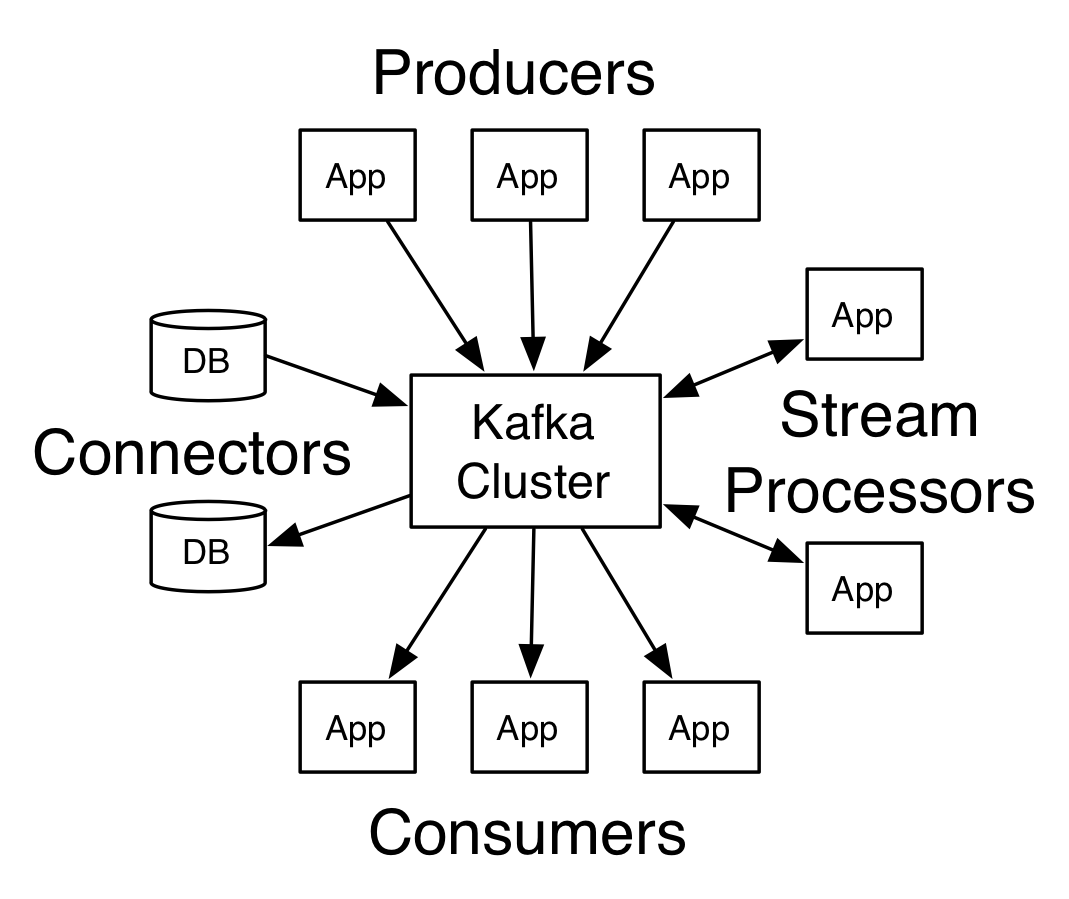
\includegraphics[scale=1.0]{figure/kafka-apis.png}
	\caption{Apache Kafka~\cite{Kafka}}
\end{figure}

Apache Kafka ist eine verteilte skalierbare Streaming Plattform.

\pnote{- Beispielkommentar}
\end{frame}


\begin{frame}
\frametitle{Eigenschaften}
Kafka ...
\begin{itemize}
	\item ist ein Message Queuing System
	\item kann Nachrichten speichern
	\item kann Nachrichten verarbeiten
	\item kann all das in Echtzeit
\end{itemize}

\pnote{- Nachrichten werden aufbewahrt}
\pnote{- können bearbeitet werden}
\pnote{- Echtzeit}
\end{frame}


\begin{frame}{Motivation}
	\begin{figure}
		\centering
		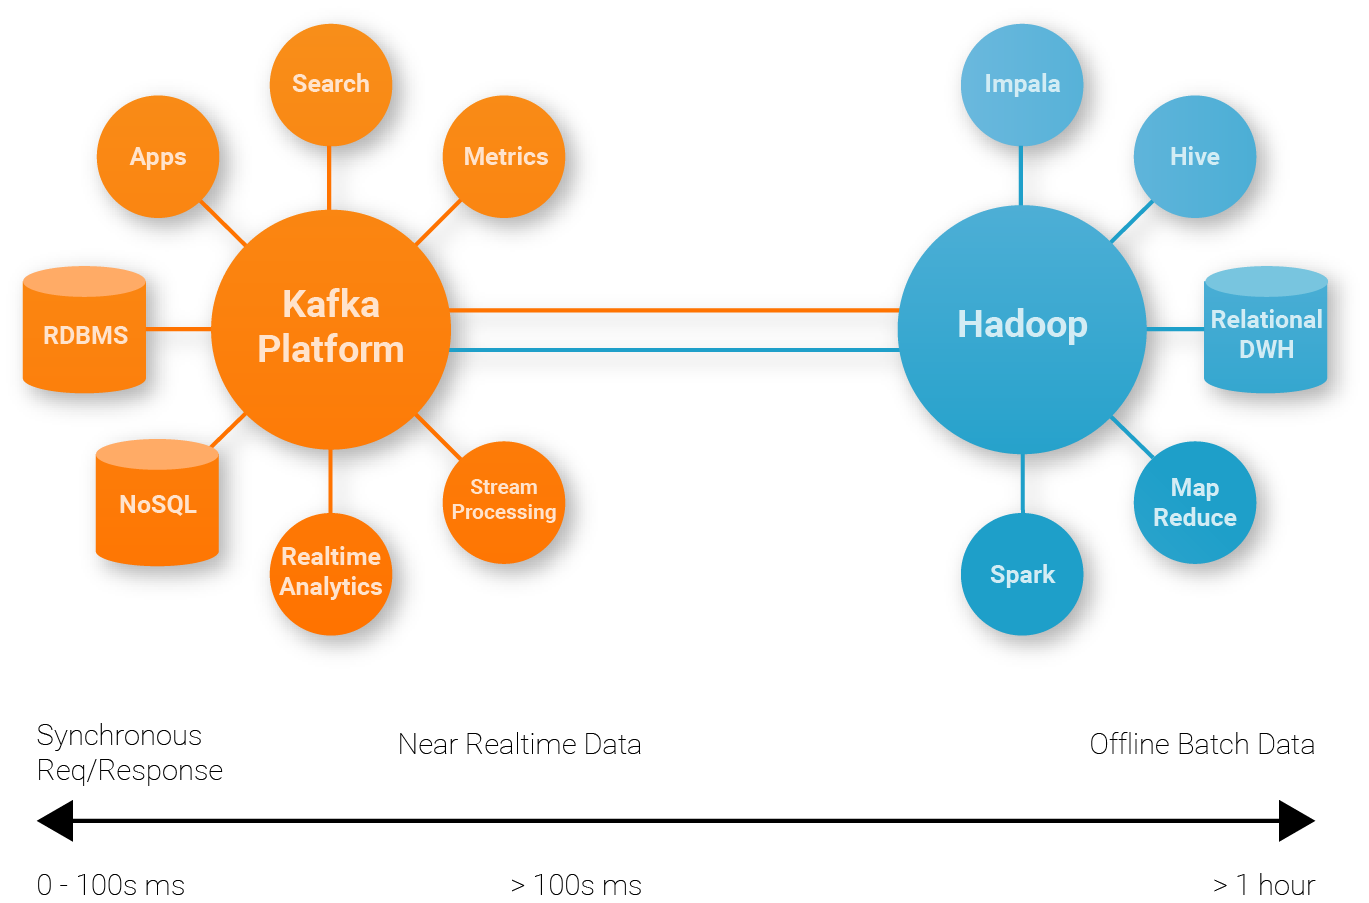
\includegraphics[scale=0.165]{figure/kafka_vs_hadoop.png}
		\caption{Kafka and Hadoop~\cite{Rao17}}
	\end{figure}
\end{frame}


\begin{frame}
\frametitle{Unternehmen und Use Cases}

\begin{tabular}{cl}
	\raisebox{-.25\height}{
\includegraphics[scale=0.2]{figure/linkedin_logo.pdf}} 
		& Operational Metrics\\~\\
	\raisebox{-.25\height}{
\includegraphics[scale=0.2]{figure/cisco_logo.pdf}} 
		& OpenSOC (Security Operations Center)\\~\\
	\raisebox{-.25\height}{
\includegraphics[scale=0.08]{figure/netflix_logo.pdf}} 
		& Real-time Monitoring and Event-processing Pipeline\\~\\
	\raisebox{-.25\height}{
\includegraphics[scale=0.2]{figure/spotify_logo.pdf}} 
		& Log Delivery System\\~\\
	\raisebox{-.25\height}{
\includegraphics[scale=0.1]{figure/twitter_logo.pdf}} 
		& Part of Storm Stream Processing Infrastructure
		
		\pnote{* Zentrale Data Pipeline }
		\pnote{- 1.4 Billarden Narichten/Tag 1400 Broker} % https://engineering.linkedin.com/blog/2016/04/kafka-ecosystem-at-linkedin
		\pnote{* OpenSecurityOperationsCenter}
		\pnote{- Als Messaging System zwischen Data Collection und Real Time Processing}
		% We currently operate 36 Kafka clusters consisting of 4,000+ broker instances for both Fronting Kafka and Consumer Kafka. More than 700 billion messages are ingested on an average day.
		\pnote{- Zum Einsammeln von Clientdaten eingesetzt}
		
\end{tabular}
\end{frame}


\subsection{Grundlagen (Queue \& Topic)}

%% Was sind Records? -> Auf Folie aufnehmen.

\begin{frame}
\frametitle{Queue}
\begin{center}
	\centering
	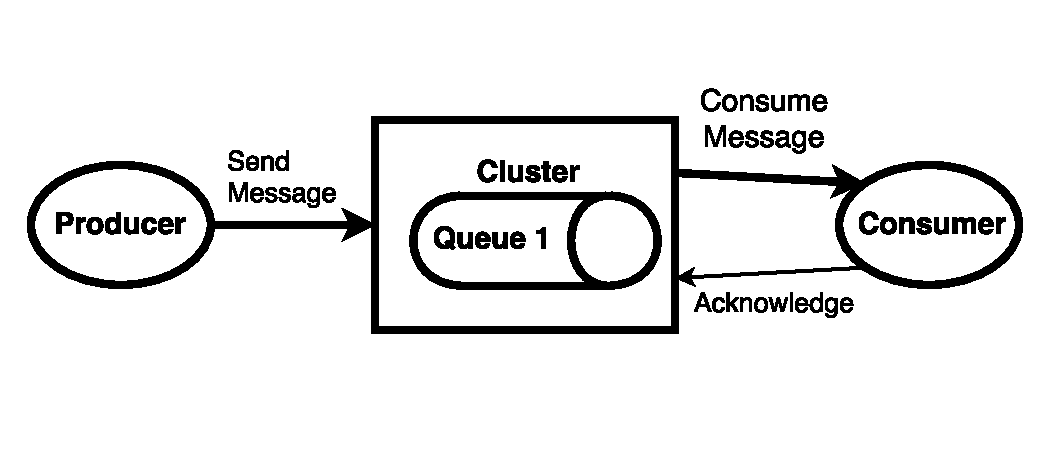
\includegraphics[scale=0.6]{figure/queue_draw.pdf}
\end{center}
\end{frame}

\begin{frame}
\frametitle{Topic}
	\centering
	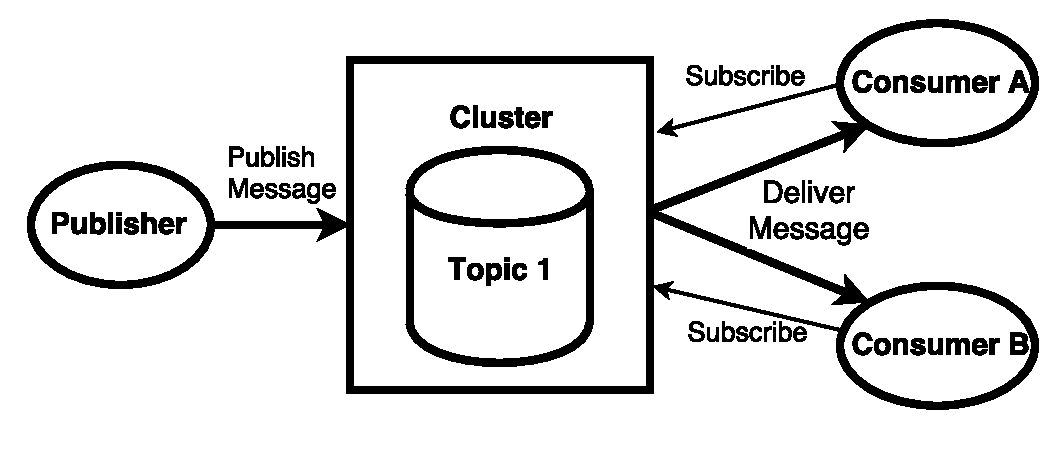
\includegraphics[scale=0.6]{figure/topic_draw.pdf}
\end{frame}

%% Messaging System
\begin{frame}
\frametitle{Zusammenfassung}

Bisher: 
\begin{itemize}
	\item Queueing
	\begin{itemize}
		\item Nachricht 1:1 Consumer
		\item Nachrichtenverarbeitung skaliert
		\item Nachricht abgerufen = Nachricht weg
	\end{itemize}
	\item Publish-Subscribe
	\begin{itemize}
		\item Nachrichten 1:N Consumer
		\item Skaliert nicht  			%Jeder bekommt die Nachricht. Daher nicht horizontal skallierbar.
	\end{itemize}
\end{itemize}
\end{frame}

\subsection{Kafka Topic}
\begin{frame}
\frametitle{Kafka Topic}
\centering
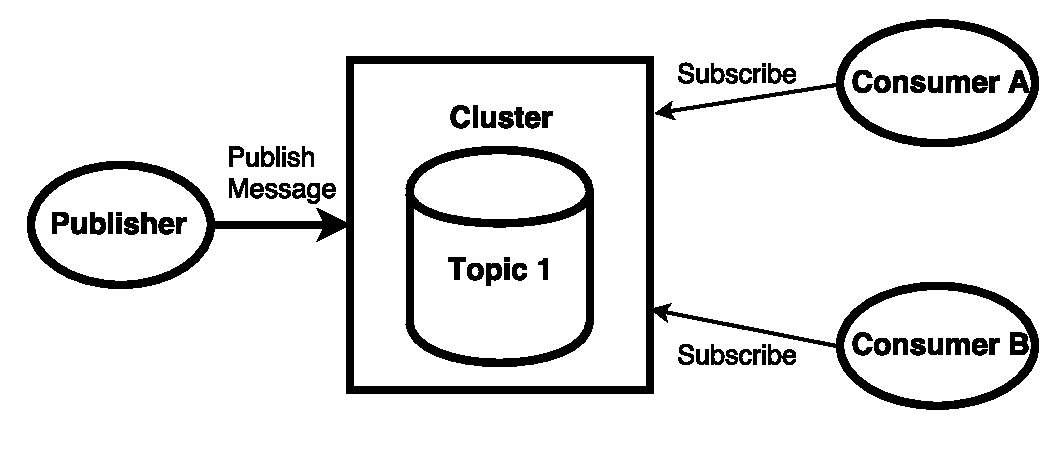
\includegraphics[scale=0.6]{figure/Kafka_topic_draw_subscribe.pdf}
\end{frame}

\begin{frame}
\frametitle{Kafka Topic}
\centering
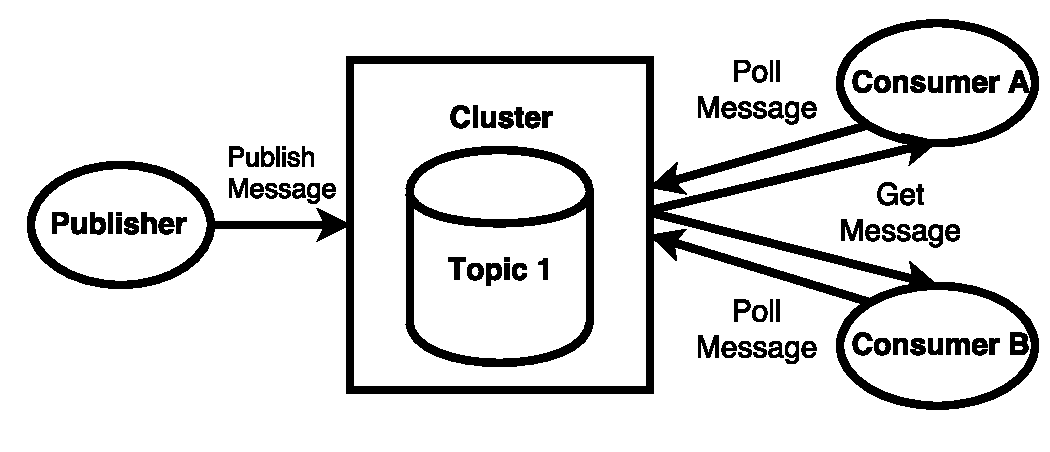
\includegraphics[scale=0.6]{figure/Kafka_topic_draw_Poll.pdf}
\pnote{* Poll verringert die Kopplung von Consumern und Producern}
\end{frame}


\begin{frame}
\frametitle{Kafka Topic}
\begin{itemize}
	\item Vereinigt klassische Queue und Pub/Sub
	\item Multi-Subscribe ($0$ bis $n$ Consumer)		% Consumergroups - n Anzahl der Partitionen
	%\item Kein Push-System
	\pnote{kein Push -> Pull}
	\item Records in Topics werden persistent gehalten
	\item Topics benötigen eine Cleanup-Policy
		\begin{itemize}
			\item Retention-Time
			\pnote{* Retention-Time: nach gewisser Zeit löschen}
			\item Retention-Size
			\pnote{* Retention-Size: ab gewisser größe löschen}
			\item Log-Compaction
			\pnote{* Log-Compaction: hält von jeder message mit dem gleichen Key die neuste Nachricht. }
		\end{itemize}
	\item Guarantees
		\begin{itemize}
			\item Reihenfolge der Records wird eingehalten
			\pnote{Nachrichten in Reihenfolge im Log wie gesendet}
			\item Consumer sehen die Einträge wie im Log gespeichert
			\item Replikations Faktor N : N-1 Serverausfälle werden toleriert
			\pnote{* Guarantees: Reihenfolgesicherung beim schreiben und lesen, Ausfall N-1 }
		\end{itemize}
\end{itemize}
\end{frame}

\begin{frame}
\frametitle{Partitionen}
	\centering
	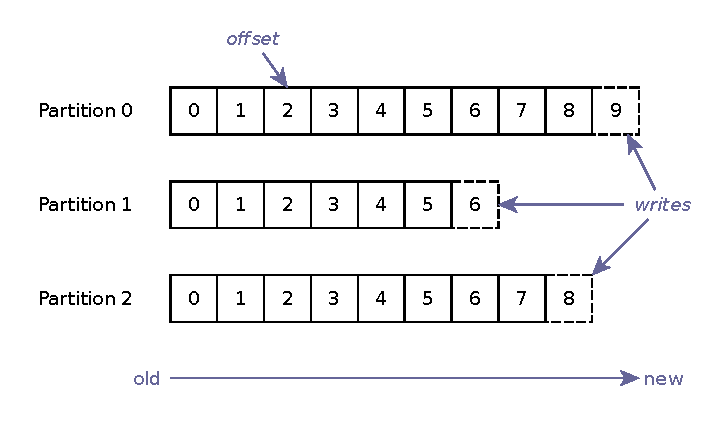
\includegraphics[scale=0.75]{figure/partitioned_log.pdf}
\end{frame}

\begin{frame}
\frametitle{Partitionen}
\centering
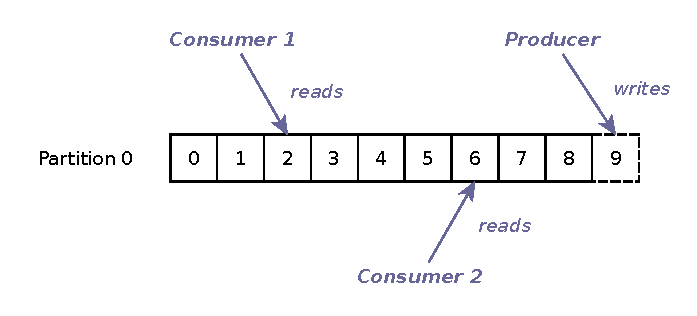
\includegraphics[scale=0.75]{figure/partition.pdf}
\end{frame}

\begin{frame}
\frametitle{Partitionen}
\begin{itemize}
	\item $1..n$ Partitionen für jedes Topic
	\item Eine Partition ist
	\begin{itemize}
		\item Geordnet
		\item Nicht-Veränderbare Sequenz von Records
		\item Records können angehängt werden
	\end{itemize}
	\item Records sind nummeriert
	\item Records werden nach Cleanup-Policy entfernt
	\item Sequentielle Abarbeitung ist Standard
	\item Sprung im Record-Log möglich
\end{itemize}
\end{frame}

\begin{frame}
\frametitle{Partitionen}
\begin{itemize}
	\item Verteilung der Partitionen ermöglicht
	\begin{itemize}
		\item Gute Skalierung
		\item Parallele Abarbeitung
	\end{itemize}
\end{itemize}
\end{frame}

\subsection{Kafka Eigenschaften}
%% Messaging System
\begin{frame}
\frametitle{Kafka als Nachrichtensystem}

\begin{columns}[T] % contents are top vertically aligned
	\begin{column}[T]{.65\textwidth} 
		\begin{itemize}
			\item Consumer Groups
			\begin{itemize}
				\item Kombiniert Queueing und Publish-Subscribe
				\item Nachrichtenverarbeitung in Gruppen
				\item Mehrere Consumer in einer Gruppe
			\end{itemize}
			\item Vorteile?
			\begin{itemize}
				\item Nachrichtenverarbeitung skaliert? % Durch Skalierung horizontal Groups und vertical mehrere consumer pro group
			\end{itemize}
			\item Reihenfolge wird eingehalten?
		\end{itemize}
	\end{column}
	\begin{column}[T]{.35\textwidth}
		\begin{figure}
		\centering
		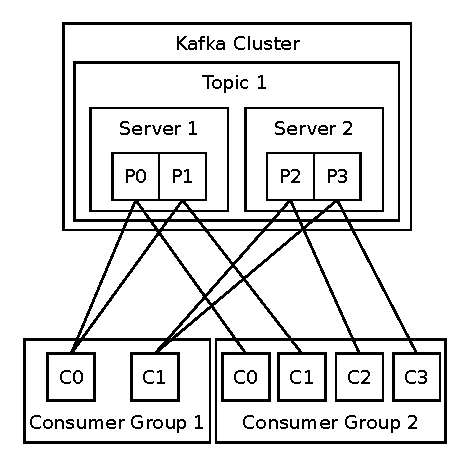
\includegraphics[scale=0.5]{figure/consumer_groups.pdf}
		\caption{Consumer Groups~\cite{Kafka}}
		\end{figure}
	\end{column}
\end{columns}



\end{frame}

%\begin{frame}
%\frametitle{Parallelität?}
%\begin{itemize}
%	\item Ordnung 
%	\begin{itemize}
%		\item Gesichert für alle Consumer Groups
%	\end{itemize}
%	\item Lastverteilung
%		\begin{itemize}
%		\item Nachricht 1x pro Consumer Group verarbeitet
%	\end{itemize}
%\end{itemize}
%
%\end{frame}

%% Storage System
\begin{frame}
\frametitle{Kafka als Datenbank}

\begin{block}{Kafka as a Storage System}
	"Kafka [is] a kind of special purpose distributed filesystem dedicated to high-performance, low-latency commit log storage, replication, and propagation." \cite{Kafka}
\end{block}


\begin{itemize}
	\item Durch Funktionalität bedingt
	\begin{itemize}
		\item Entkopplung  von Cunsumer und Producer sorgt für Speicherbedarf
	\end{itemize}
	\item Daten werden repliziert
	\begin{itemize}
		\item Bestätigungsmechanismen sind vorhanden
		\item Wird erst bestätigt, wenn Replication abgeschlossen ist
	\end{itemize}
\end{itemize}

\end{frame}

%\begin{frame}
%\frametitle{Kafka als Datenbank - 2}

%\begin{itemize}
%	\item Performanz bei steigender Datenmenge gleich
%	\item Eigenschaften:
%	\begin{itemize}
%		\item Hohe Performanz
%		\item Geringe Latenz %% Für Commit Log Storage
%		\item Replikation
%		\item Weiterleitung %% Von Nachrichten
%	\end{itemize}
%\end{itemize}
%\end{frame}

\begin{frame}
\frametitle{Kafka für Stream Processing}

\begin{itemize}
	\item Anforderung: Streamverarbeitung in \textit{Echtzeit}!
	\item Ein Stream Processor ...
	\begin{itemize}
		\item nimmt kontinuierlich Daten aus einem \textit{Input} Topic,   % Shipments
		\item bearbeitet die Daten und % Preisanpassungen berechnen
		\item schreibt kontinuierlich Daten in ein \textit{Output} Topic % Preisänderungen veröffentlichen
	\end{itemize}
\end{itemize}

\end{frame}


\begin{frame}
\frametitle{Kafka für Stream Processing - Stream API}

\begin{itemize}
	\item \texttt{Stream API} wird für nicht-triviales Stream Processing angeboten,
	z.B. zur Aggregation oder Joins von Streams. 
	\item \texttt{Stream API} unterstützt
	\begin{itemize}
		\item \textit{Exactly-once} Verarbeitung von Daten
		\item Statusbehaftete Operationen, wie Joins und Aggregationen über Bereiche
		\item Erneute Verarbeitung von Daten, wenn sich die Operation ändert
		\item \textit{One-record-at-a-time Processing}, um Verarbeitungs"-latenz im Milli"-sekunden"-bereich garantieren zu können
	\end{itemize}
\end{itemize}

%The streams API builds on the core primitives Kafka provides: it uses the producer and consumer APIs for input, uses Kafka for stateful storage, and uses the same group mechanism for fault tolerance among the stream processor instances.
\end{frame}

\subsection{Performance}
\begin{frame}{Performance}
	\centering
	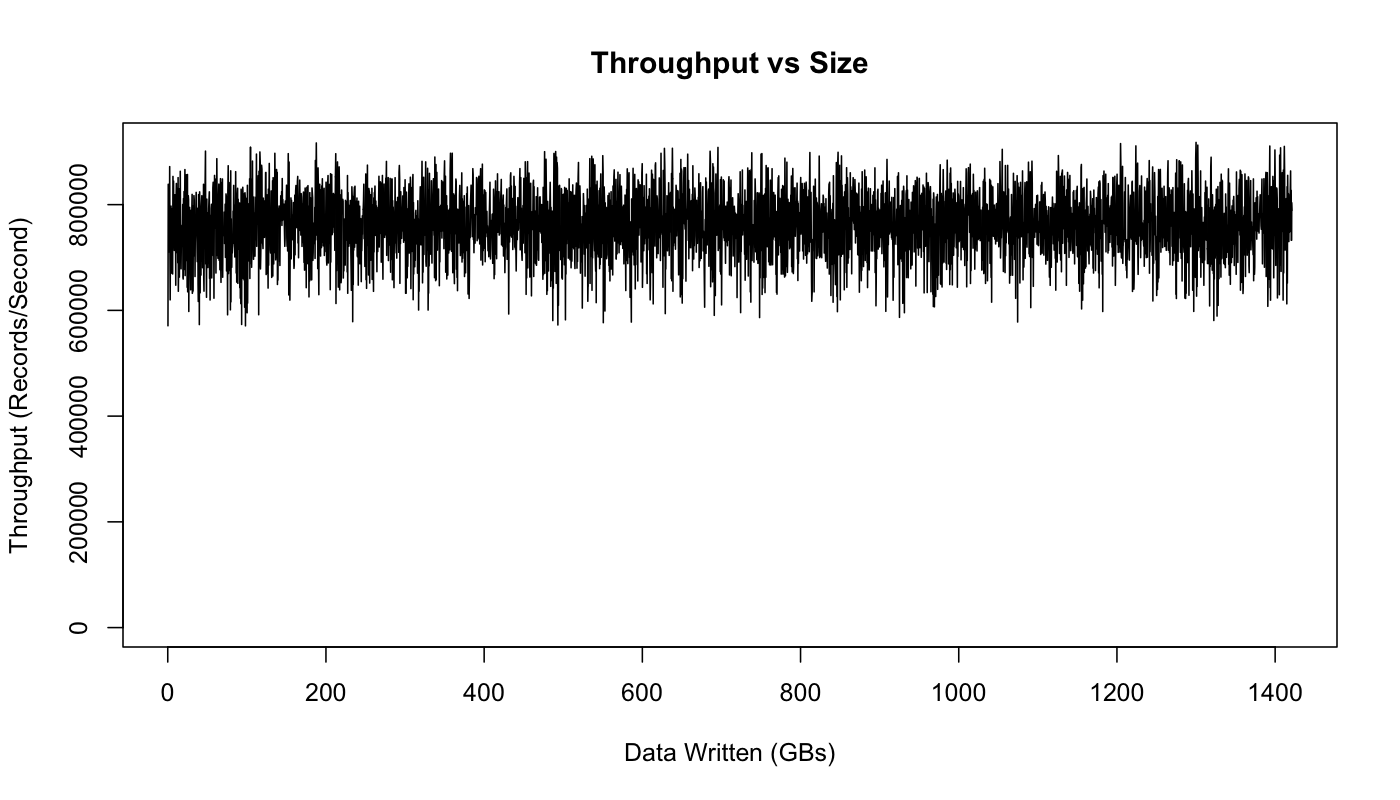
\includegraphics[scale=0.2]{figure/throughput_vs_size_0.png}

	\pnote{- Don't fear the filesystem}
	\pnote{-- Weiterentwickluing der Festplatten und Optimierungsmöglichkeiten}	
	\pnote{-- Ensure linear write disk I/O -> können stark vom OS optimiert werden (read-ahead, write-behind)}
	\pnote{-- Batching together small bits of data}
	\pnote{}
	\pnote{- Kafka kann O(1)}
\end{frame}

\begin{frame}
\frametitle{Zusammenfassung}

% Wie verpacken?
%By combining storage and low-latency subscriptions, streaming applications can treat both past and future data the same way. That is a single application can process historical, stored data but rather than ending when it reaches the last record it can keep processing as future data arrives. This is a generalized notion of stream processing that subsumes batch processing as well as message-driven applications.

%Likewise for streaming data pipelines the combination of subscription to real-time events make it possible to use Kafka for very low-latency pipelines; but the ability to store data reliably make it possible to use it for critical data where the delivery of data must be guaranteed or for integration with offline systems that load data only periodically or may go down for extended periods of time for maintenance. The stream processing facilities make it possible to transform data as it arrives.

\begin{itemize}
	\item geeignet für:
	\begin{itemize}
		\item   % Shipments
		\item Bearbeitet die Daten % Preisanpassungen berechnen
		\item Schreibt kontinuierlich Daten in ein Topic % Preisänderungen veröffentlichen
	\end{itemize}
\end{itemize}

\end{frame}